%% The following is a directive for TeXShop to indicate the main file
%%!TEX root = diss.tex

\chapter{Experimental Techniques}
\label{ch:exptech}

In this chapter, three \acf{SPM} techniques will be discussed in detail, including discussion of the underlying physical principles, methods of operation, and analysis of experimental data.



%%%%%
\section{Scanning tunnelling microscopy}

\Acf{STM} was invented in 1981 by Gerd Binning and Heinrich R\"ohrer at IBM, and was the first example of a scanning probe microscope \citep{binnig1982surface}. The \ac{STM} gives atomic resolution topographic maps of the electronic structure of a conductive sample by employing quantum tunnelling between the sample and a conductive tip, controlled by sub-nanometre precise piezoelectric motors. As seen in \autoref{fig:exptech:stmsetup}, a sharp tip is brought close to a sample, with tip-sample distances ($z$) on the order of 1--\SI{10}{\angstrom}. A bias voltage difference ($V_b$) is in place between the electrodes, driving the directional quantum tunnelling of electrons through the vacuum potential barrier between the tip and the sample. A small but detectable tunnelling current ($I_t$), typically on the order of picoamperes, goes through a preamplifier and is transduced into a voltage signal, which can then be fed into a control system.

\begin{figure} [h]
    \centering
    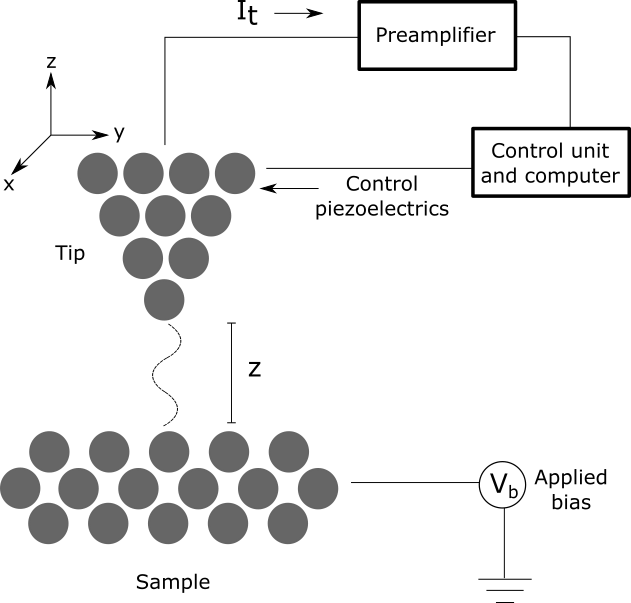
\includegraphics[width=0.65\textwidth]{pictures/stm_diagram.png}
    \caption{Schematic of STM system.}
    \label{fig:exptech:stmsetup}
\end{figure}

\sloppy An approximation of the tunnelling current could be gathered from a \ac{1D} one particle model (\autoref{fig:exptech:wkb}). The solutions of the Schr\"odinger equation in the tip and sample regions would be oscillatory free-electron wave functions\footnote{Electrons in a metal are assumed behave like free particles.}, while inside the barrier would give wave function $\psi(z) \propto e^{-kz}$, with $k^2 = 2m({V_B(z,V_b) - E})/\hbar^2$ where $V_B(z,V_b)$ is the barrier potential and $E$ is the energy of the tunnelling electron. For electrons with energies high enough and tip-sample distance $z$ small enough, the wave function would be non-zero on the other side of the barrier. From the \ac{1D} \ac{WKB} approximation, the probability of transmission is
\begin{equation} \label{eq:exptech:transfcn}
T(z,E,V_b) = \exp{\left(-2\int_{z_1} ^{z_2} k dz \right)} = \exp{\left(-2  \int_{z_1}^{z_2} \sqrt{\frac{2m}{\hbar^2}(V_B(z,V_b) - E)} dz \right)}.
\end{equation}
The barrier potential is unknown, and is often assumed be a trapezoidal barrier, as shown in \autoref{fig:exptech:wkb}. For experimental analysis, the trapezoidal barrier is further approximated by a rectangular barrier of height $V_B(V_b) = (\Phi_t + \Phi_s + eV_b)/2$. % For a constant bias voltage in \ac{STM}, we have $I_t \propto e^{-2kz}$. The tunnelling current is extremely sensitive to changes in $z$, dropping off exponentially with increasing tip-sample distances. This sensitivity allows for picometre height resolution, while the atomically sharp tip allows for sub-nanometre lateral resolution imaging.


\begin{figure} [t]
    \centering
    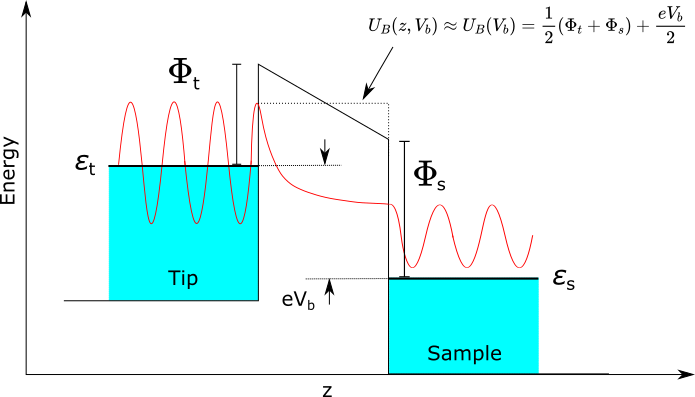
\includegraphics[width=\textwidth]{pictures/wkb.png}
    \caption{Schematic of 1D tunnelling between tip and sample. Wave functions in the tip and sample are oscillatory, and exponentially decaying in the vacuum barrier. A positive bias allows electrons under the tip Fermi energy $\varepsilon_t$ to tunnel into states above the sample Fermi energy $\varepsilon_s$.
    Trapezoidal barrier is often approximated with a constant potential based on the average work function and the bias energy.}
    \label{fig:exptech:wkb}
\end{figure}


There are two modes of \ac{STM} operation: the constant height, and the constant current mode. In both modes, the bias voltage is held constant. In constant height mode, the tip-sample distance is held constant while the tip is rastered across the sample. The corresponding fluctuations in the tunnelling current is measured as a function of the spatial variables. A drawback of this mode is the possibility of crashing the tip into the sample due to tall features on the surface, damaging both the tip and the sample. Alternatively, constant current mode holds the tunnelling current constant by using a feedback loop to adjust the tip height as it scans across the sample. In this case, the tip height is recorded as a function of the lateral $(x,y)$ positions of the tip, giving a tunnelling current isosurface plot (\autoref{fig:exptech:stmexample}). All \ac{STM} images presented in this thesis are obtained in constant current mode.

\begin{figure} [h]
    \centering
    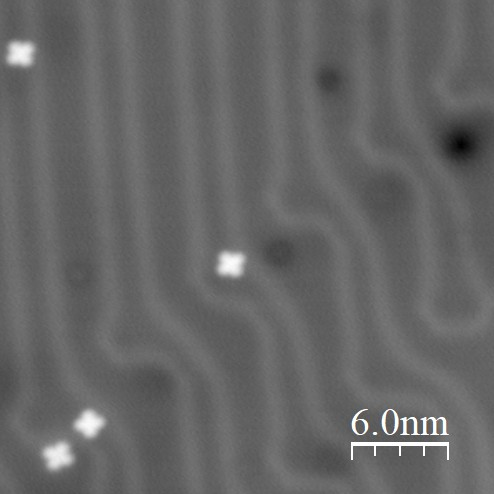
\includegraphics[width=0.5\textwidth]{pictures/f8znpc_au111_-2p5V_2pA.jpg}
    \caption{Constant current STM image (\stmparams{30}{30}{-2.5}{2}). \ch{F8ZnPc} molecules on Au(111) with herringbone reconstruction. Defects and contaminants observed on surface.}
    \label{fig:exptech:stmexample}
\end{figure}

% also talk about how to interpret the data, not exactly a physical topography
It is important to note that an \ac{STM} image should not be interpreted as a physical topography, but rather the electronic topography of the surface at a given bias. This is because the tunnelling current is dependent on the \ac{DOS} of the sample and the tip. A larger `height' indicates a higher density of states at a given point and bias, and not necessarily a taller feature on the sample. More details on the tunnelling current is given in \autoref{sec:exptech:sts}.




%%%%%
\section{Scanning tunnelling spectroscopy}
\label{sec:exptech:sts}

\Acf{STS} is a technique similar to \ac{STM}, but allows for energetic resolution of the \ac{LDOS} of the sample. At a point over the sample, the tip is held at a constant height and the current feedback loop is turned off. The tunnelling current is then measured as the bias between tip and sample is swept across a range of values. For studying organic molecules, the bias typically goes up to $\sim \SI{3}{V}$ depending on the molecular stability and the energy at which the orbital features are found.

The relationship between the current signal, $I(V)$, and the \ac{LDOS} can be understood by returning to the \ac{1D} tunnelling model (\autoref{fig:exptech:stsldos}). The tip is assumed to have a constant density of states. The bias voltage shifts the energy of the electrons in the tip relative to those of the sample. At positive biases, the Fermi level\footnote{The Fermi level is the electrochemical potential of the material, or the energy at which there is 50\% state occupation at finite temperatures. This is not to be confused with the Fermi energy, which is defined for $T=0$K. The terms will be used interchangeably, as our experimental condition is close to absolute zero.} of the tip shifts up, allowing electrons to tunnel into the unoccupied states of the sample. Conversely, at negative biases, the Fermi level of the tip shifts down, allowing electrons to tunnel from the occupied sample states into the tip. Changes in the sample density of states $\rho_s(E)$, both occupied and unoccupied, will open new tunnelling channels that are reflected in changes in the measured $I(V)$. More details on the tunnelling current and the recovery of the density of states are described in the below sections.

\begin{figure} [h]
    \centering
    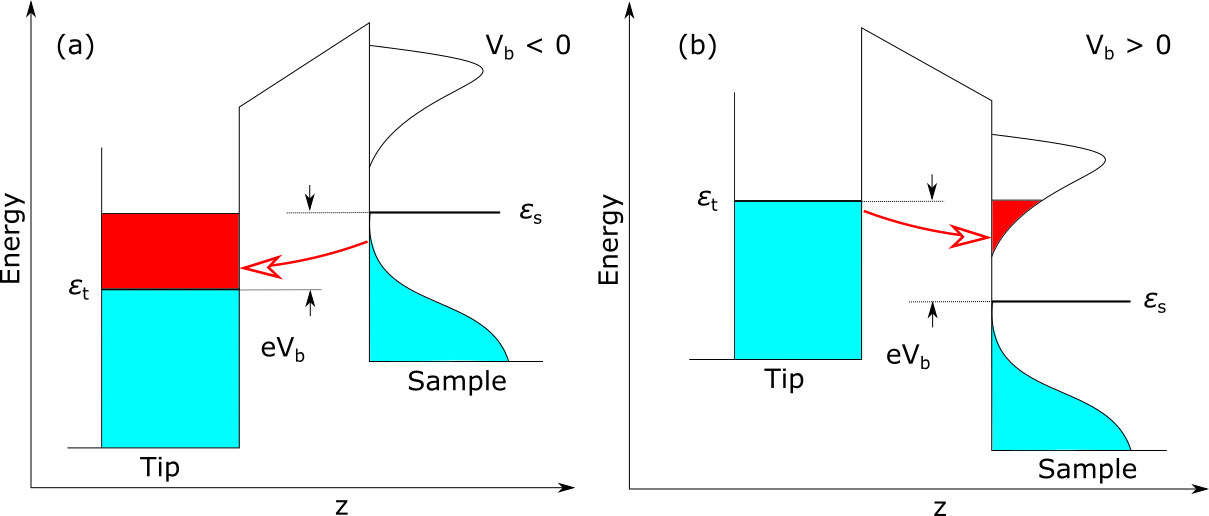
\includegraphics[width=\textwidth]{pictures/sts_ldos.png}
    \caption{Schematic showing the tunnelling process as a function of bias voltage. \textbf{(a)} At negative bias voltage, the tip Fermi energy is below the sample Fermi energy. The resulting current arises from electrons of the occupied sample LDOS tunnelling into the tip. \textbf{(b)} For positive bias voltages, the reverse process occurs, and electrons in the tip tunnel into the unoccupied sample LDOS.}
    \label{fig:exptech:stsldos}
\end{figure}

The technique can be further extended by performing \ac{STS} pixel-by-pixel in a grid, giving a spatial map of the \ac{LDOS} over an area of the sample. This is done in conjunction with \ac{STM}, with the tip pausing at grid points for \ac{STS} spectra, before resuming the \ac{STM} scan. The added time for pixel-by-pixel spectra means that \ac{STM}/\ac{STS} grids can take hours to complete, during which changes in the sample or the tip can affect measurements. 


\subsection{Tunnelling theory}
% \FIXME{Add Bardeen, Tersoff and Hamann, Feuchtwang, Caroli et al., JB Pendry, Gottlieb and Wesoloski citations.}
In order to extract quantitative information from \ac{STS}, we must understand the theory of quantum tunnelling, and its application to the tip-sample configuration of the experiment. The first theoretical formulation of many particle tunnelling was developed by \textit{Bardeen} in 1960, using what was called a `transfer Hamiltonian' \citep{PhysRevLett.6.57}. It was then applied to \ac{STM}/\ac{STS} by \textit{Tersoff and Hamann} \citep{0957-4484-17-8-R01,tersoff1985theory}. 

It is important to note that Bardeen's formulation is an approximation and does not take into account many-body effects, strong tip-sample interactions, and strong tunnelling. To date, the most rigorous analytic tunnelling theory is formulated using \acp{NEGF}, first developed by \textit{Feuchtwang} and later expanded upon by \textit{Pendry et al.}, which can address the short-comings of the transfer Hamiltonian \citep{feuchtwang1974tunneling, pendry1991theory} . However, there is currently no method to utilise \acp{NEGF} to extract \ac{DOS} from experimental \ac{STS} data. Furthermore, the \ac{NEGF} tunnelling theory has been demonstrated to be reducible to Bardeen's tunnelling theory, and thus, this section will discuss the transfer Hamiltonian approach to tunnelling, as discussed in reference \citep{0957-4484-17-8-R01}.

% taken from Guide on tunnelling Theory
In assuming that the tip and sample are independent, with weak interactions between them, we can define the sample and tip Hamiltonians separately as
\begin{align}
H_{s}\psi(\pmb{r}) &= -\frac{\hbar^2}{2m} \nabla^2 \psi(\pmb{r}) + V_{s}(\pmb{r}) \psi(\pmb{r}), \\
H_{t}\phi(\pmb{r}) &= -\frac{\hbar^2}{2m} \nabla^2 \phi(\pmb{r}) + V_{t}(\pmb{r}) \phi(\pmb{r}) ,
\end{align}
where $V_s$(\pmb{r}) and $V_t$(\pmb{r}) are the sample and tip potentials, respectively; $\psi(\pmb{r})$ and $\phi(\pmb{r})$ are eigenstates bounded to the sample and tip, respectively. We can also define a Hamiltonian of the entire system responsible for the transfer of electrons between the tip and sample (the so called `transfer Hamiltonian')
\begin{equation} \label{eq:exptech:transH}
H\Psi = - \frac{\hbar^2}{2m} \nabla^2 \Psi + V(\pmb{r}) \Psi \quad \textrm{where} \quad V(\pmb{r}) = 
\begin{cases}
V_t(\pmb{r}) & \textrm{ in tip} \\
V_t(\pmb{r}) + V_s(\pmb{r}) & \textrm{ in barrier} \\
V_s(\pmb{r}) & \textrm{ in sample}
\end{cases},
\end{equation}
where $\Psi(\pmb{r})$ are the eigenstates of the transfer Hamiltonian, and the potentials of the tip and sample only overlap in the vacuum barrier region.

\sloppy Consider an initial sample state\footnote{The spatial $\pmb{r}$ dependence of the states are implied, and dropped from the notation.} $\psi(t=0)$ which satisfies the eigenvalue equation $H_{s}\psi(0) = \epsilon \psi(0)$. When tunnelling is weak enough, then for some small time $t$ the sample states would be given by $\psi(t) = e^{-itH_{s}/\hbar} \psi(0) = e^{-it\epsilon/\hbar} \psi(0) $. For all $t$, assuming that tunnelling is weak, we expand over the tip states $\phi_k$ satisfying the eigenvalue equation $H_{t}\phi_k = \xi_k \phi_k$
\begin{equation} \label{eq:exptech:state}
\psi(t) = e^{-it\epsilon/\hbar} \psi(0) + \sum_k a_k(t) \phi_k,
\end{equation}
where $a_k$ are coefficients of the expansion. Since there is no tunnelling initially, there would be no contribution from the tip state, and for all $k$ the coefficients vanish at $t=0$. By approximating $a_k(t)$, we can take the time derivative to look at the rate of `transfer' from the initial sample state to the tip state, and from that the tunnelling current.

By plugging the state (\autoref{eq:exptech:state}) into the time-dependent Schr\"odinger equation of the transfer Hamiltonian (\autoref{eq:exptech:transH}), and separately taking the time derivative, we have two expressions for $\frac{\partial \psi}{\partial t}$. Equating gives us
\begin{equation}
i\hbar \sum_k \frac{d}{dt} a_k(t) \phi_k = e^{-it\epsilon / \hbar} (H-H_{s})\psi(0) + \sum_k a_k(t) (\xi_k \phi_k + (H-H_{t})\phi_k),
\end{equation}
where $H$ is the transfer Hamiltonian, and $\xi_k$ are the eignenenergies of the tip states. Taking the inner product with $\phi_j$, for any $j$-th tip state
\begin{equation} \label{eq:exptech:scatteringprob}
i\hbar \frac{d}{dt} a_j(t) = e^{-it\epsilon/\hbar} \Bra{\phi_j}H-H_{s} \Ket{\psi} + \xi_j a_j(t) + \sum_k a_k(t) \Bra{\phi_j} H - H_{t} \Ket{\phi_k}.
\end{equation}

Due to weak tunnelling, for a little while ($t \ll 1$), $a_j(t)$ is the only non-zero coefficient, and the last term of \autoref{eq:exptech:scatteringprob} vanishes. The resulting differential equation has solutions
\begin{equation}
a_j(t) =  \frac{e^{-it\epsilon/\hbar} - e^{-it\xi_j/\hbar}}{\epsilon - \xi}  \Bra{\phi_j} H-H_{s} \Ket{\psi}.
\end{equation}
For rate of scattering from the sample into the tip as a result of the transfer Hamiltonian (\autoref{eq:exptech:transH}), calculate the total $\sum_k \abs{a_k(t)}^2$ and take the time derivative
\begin{equation}
\frac{d}{dt}\sum_k |a_k(t)|^2 = \frac{d}{dt}  \sum_k \frac{t^2}{\hbar^2}\textrm{sinc}^2 \left(\frac{t(\xi_k - \epsilon)}{2\hbar} \right) | \Bra{\phi_k} H-H_{s} \Ket{\psi}  | ^2.
\end{equation}

For sufficiently large $t$, the sinc function can be approximated as the Dirac $\delta$-function. For a continuous \ac{DOS}, the summation over $k$ becomes an integral over all energies, and the integral can be evaluated

\begin{align}
\frac{d}{dt}\sum_k |a_k(t)|^2 &\approx  \frac{d}{dt}  \int_{-\infty}^\infty dE \left[ \frac{\pi t^2}{\hbar^2} \delta \left(\frac{t(E - \epsilon)}{2\hbar} \right) | \Bra{\phi_E} H-H_{s} \Ket{\psi}  | ^2 \right], \\
&\approx  \frac{2\pi }{\hbar} \rho_t(\epsilon) \abs{\mathfrak{M}}^2,
\end{align}
where $\rho_t(\epsilon)$ is the tip density of states near $\epsilon$, the eigenenergy of the sample state $\psi$. The equation above is also known as Fermi's Golden Rule. The matrix elements $\abs{\mathfrak{M}}^2 = \abs{\Bra{\phi_\epsilon} H - H_s \Ket{\psi}}^2$ is the transition probability of the sample state into a tip state near $\epsilon$, denoted as $\phi_\epsilon$.

To get the tunnelling current, we look to the work of Tersoff and Hamann, considering tunnelling from either sides of the junction. We continue to assume independent sample and tip and weak tunnelling, such that the addition or removal of electrons do not greatly affect the chemical potentials of the tip and sample, $\mu_t$ and $\mu_s$ respectively. We will also assume a low bias so that band-bending phenomena is negligible.

In these limits, the statistics of the electrons are governed by the Fermi-Dirac distribution: at temperature $T$ and chemical potential $\mu$, the probability finding an electron at energy $E$ is $F_{\mu, T}(E) = ({e^{(E-\mu)/k_BT} +1})^{-1}$. The tunnelling of electrons \emph{from} a \emph{filled} sample state $\psi_n$ with energy $\epsilon_n$ into an empty tip state would be
\begin{equation} \label{eq:exptech:Is->t}
    I_{s\rightarrow t} = \frac{2\pi e}{\hbar} \sum_n F_{\mu_s, T}(\epsilon_n) (1-F_{\mu_t, T}(\epsilon_n))  \rho_{t}(\epsilon_n) \abs{\mathfrak{M}}^2 
\end{equation}
where $e$ is the elementary charge. The tunnelling of electrons \emph{into} an \emph{empty} sample state $\psi_n$ from filled tip states near energy $\epsilon_n$ would be 
\begin{equation} \label{eq:exptech:It->s}
    I_{t\rightarrow s} = \frac{2\pi e}{\hbar} \sum_n (1-F_{\mu_s, T}(\epsilon_n))   F_{\mu_t, T}(\epsilon)  \rho_{t}(\epsilon_n) \abs{\mathfrak{M}}^2 .
\end{equation}

% Since the bais was defined relative to the sample, the current from the tip to sample is defined as positive, and from the sample to tip as negative. 
The difference between the expressions in \autoref{eq:exptech:Is->t} and \ref{eq:exptech:It->s} will give the total tunnelling current. Rewritting the total current by referencing the energy $\epsilon_n$ with respect to the Fermi level of the sample, which is biased lower than the tip energy by $eV_b$, we have
\begin{equation} 
I = \frac{2\pi e}{\hbar}\sum_n f(\epsilon_n, V_b) \rho_{t}(\epsilon_n) \abs{\mathfrak{M}}^2,
\end{equation}
where $ f(\epsilon_n,V_b) = F_{\mu_t=0,T}(\epsilon_n-eV_b) - F_{\mu_s=0,T}(\epsilon_n)$. Note that the Fermi-Dirac equations no longer depend on the chemical potentials of the sample and tip, as they are already accounted for by the bias $eV_b = \mu_t - \mu_s$. 

The entire expression can be approximated by an integral
\begin{equation}
    I \approx \frac{2\pi e}{\hbar} \int_{-\infty}^\infty dE f(E,V_b) \rho_t(E)\rho_s(E) T(E,V_b,z),
\end{equation}
where the matrix elements are approximated by averaging over the sample states $\phi$ near the energy $E$, giving $\abs{\mathfrak{M}}^2 \approx T(E,V_b,z) \rho_s(E)$, where $T(E,V_b,z)$ is the transmission probability in \autoref{eq:exptech:transfcn} .

Taking the limit of $T \rightarrow \SI{0}{\kelvin}$, the Fermi-Dirac equations become Heaviside functions, and $f(E,V_b) = 1$ for $E \in [0,eV_b]$, and 0 elsewhere. Physically, only electrons with energies between the Fermi levels of the sample and tip contribute to the tunnelling current; the expression for the tunnelling current becomes
\begin{equation} \label{eq:exptech:tersoffcurrent}
I_{T \rightarrow 0K} \approx \frac{2\pi e}{\hbar} \int_{0} ^{eV_b} dE \rho_{t}(E) \rho_{s}(E) T(E,V_b,z).
\end{equation}

It is important to remember the limits in which this equation is valid. From Bardeen's formalism, we assume (1) no electron-electron interaction, (2) independent tip and sample states, and (3) weak tunnelling. In Tersoff and Hamann's analysis, we further assume (4) Fermi-Dirac statistics, (5) first-order \ac{WKB} tunnelling, (6) low temperatures, and (7) negligible band-bending effects. In general, these conditions hold when the tip and sample are sufficiently far apart, and bias between the two are sufficiently low.


\subsection{Normalisation of $dI/dV$}

From the Tersoff and Hamann equation, we can extract the density of states of the sample from the \ac{STS} spectra. In \autoref{eq:exptech:tersoffcurrent}, the current is a convolution of the \ac{DOS} of the tip and sample, and the transmission probability. Assuming that the \ac{DOS} of the tip is featureless, and equal to unity
\begin{equation}
I \propto \int_0 ^{eV} dE \rho_s(E) T(E,V,z) .
\end{equation}
In taking the derivative with respect to the bias voltage\footnote{The subscript in $V_b$ is implied. The $V$ is no longer used to discuss potential barriers, and is used exclusively to indicate the bias voltage.}, we obtain the differential conductance
\begin{equation} \label{eq:exptech:didv}
\frac{dI}{dV} \propto e \rho_s(E=eV) T(E=eV,eV,z) + e \int_0^{eV} dE \rho_s(E) \frac{dT(E,V,z)}{dV}  .
\end{equation}

A commonly used form for the \ac{DOS} of the sample, $\rho_s(E) \propto dI/dV $, where, for small enough biases ($\sim \SI{10}{\milli\electronvolt}$), the integral term in \autoref{eq:exptech:didv} is ignored \citep{feenstra1993methods}. However, for studies of organic semiconductor molecules, features are often found at larger biases ($\sim 1$--$\SI{3}{\electronvolt}$), which would be obscured by the exponential form of the transmission probability (\autoref{eq:exptech:transfcn}). To eliminate the exponential dependence, the differential conductance can be `normalised' with the conductance  \citep{feenstra1987atom}
\begin{equation} \label{eq:exptech:normdidv}
\frac{dI/dV}{I/V} = \frac{\rho_s(eV) + \int_0 ^{eV} dE \frac{\rho_s(E)}{T(E=eV,eV)} \frac{dT(E,V,z)}{dV}}{ \frac{1}{eV} \int_0^{eV} dE \rho_s(E) \frac{T(E,eV)}{T(E=eV,eV)}}.
\end{equation}
In this form, the transmission probability appears in ratios with itself, qualitatively canceling the exponential form. The normalised differential conductance gives the $\rho_s(eV)$ with some ``background" term arising from interactions of the wavefunction with the electric field in the junction.

However in \autoref{eq:exptech:normdidv}, divergences arise when we consider $V=\SI{0}{\volt}$ or $I= \SI{0}{\ampere}$. To mitigate this, a small constant term can be added to the conductance without significantly modifying the normalisation term \citep{prietsch1991structural}
\begin{equation}
    \overline{I/V} = \sqrt{(I/V)^2 + c^2},
\end{equation}
where for constant $c\ll I/V$ we would have $\overline{I/V} \approx I/V$ to the first order. For \ac{STS} data analysed in this thesis, all \ac{DOS} is approximated by $ (dI/dV) / (\overline{I/V})$.

%%%%%
\section{Scanning tunnelling microscopy luminescence}

% allows us to probe the excited states of molecules on surface
In the \ac{STM} setup, an optical system can be integrated to allow for detection of tunnelling induced luminescence. This mode of operation is known as \acf{STML}. The tip acts as a source of electrons and holes that can locally excite photon emission from the sample \citep{gimzewski1988photon}, thus allowing the near-field study of luminescence from nanoscale structures on metals, semiconductors, and molecules \citep{Qiu2003}. The intensity and spectral distribution of the photons provide information on electron-hole transport and the optical properties of the material, as well as inelastic tunnelling processes which would otherwise be undetectable in \ac{STM} or \ac{STS}. Additionally, with organic semiconductor molecules, chemical and vibrational signatures can be seen in the photoemission spectra, particularly in the visible and infrared ranges \citep{Qiu2003,Wu2008}.

To perform \ac{STML}, there must be optical access to the tip-sample junction of the \ac{STM}. A lens mounted to the microscope head and focused at the junction, which is closely approximated to be a point source, collimates the emission. An optical path through several windows and viewports allows the photons to exit the microscope and refocused by an exterior lens into a detector, such as a spectrometer. 

% The spectrally resolved photons give information on the excited states and vibrational modes of the molecule. Combined with the high spatial resolution of the \ac{STM}, emission and absoprtion spectroscopy can be carried out on single molecules in the optical near-field regime. With \ac{STML}, a real-space nanoscale understanding of the electromagnetic coupling of \ac{OLED} and \ac{OPV} molecules can be achieved.

Emission from the tunnelling junction can be described by two main processes: (1) the excitation of the free electron gas in the metallic substrate, and (2) the fluorescence of a quantum confined system---such as an organic semiconductor molecule. The subsequent sections will describe both processes in further detail. 


\subsection{Plasmon emission}

The first observations of tunnelling induced luminescence were seen in metal-oxide-metal junctions in 1976, by Lambe and McCarthy \citep{lambe1976light}. Later experiments on metal and semiconductor surfaces demonstrated that the same effect can be seen in \ac{STM}. While there are other proposed mechanisms, the emission is generally attributed to the decay of plasmons excited by \acf{IET} processes \citep{berndt1991inelastic}.

Inelastic processes in tunnelling accounts for about 1\% of the total current, making this process difficult to measure in \ac{STM} and \ac{STS} \citep{novotny2012principles}. In \ac{IET}, the electrons or holes lose a fraction of energy during tunnelling, exciting localised charge oscillations in the substrate, also known as plasmons. Plasmons at the interface between the metallic substrate and the vacuum can couple to the electromagnetic field, becoming \acp{SPP}, which then decay into photons.\footnote{Although no plasmons are physically emitted, due to the origin of the emissions, I will refer to the photons as ``plasmon emission.''} 

% In some models, the inelastic process occurs \emph{after} elastic tunneling, when the electron thermalises (release energy) which then excites the \ac{SPP}. This is known as \acf{HET}. In metals and indirect-gap semiconductors, \ac{HET} is negligible compared to \ac{IET}, with theoretical estimates putting the quantum efficiency, the photons emitted per charge carrier, of \ac{IET} two orders of magnitude higher. However in direct-gap and organic molecular semiconductors, \ac{HET} may be the primary mechanism for luminescence.

\begin{figure} [h]
    \centering
    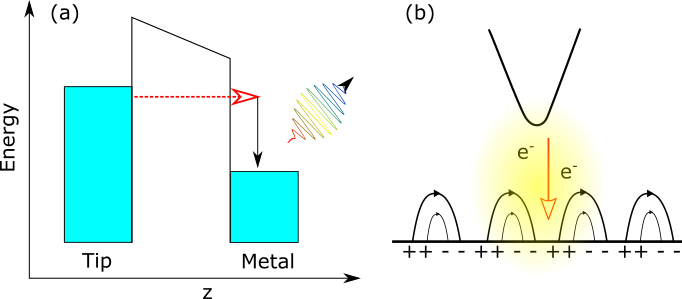
\includegraphics[width=\textwidth]{pictures/spp_emission.png}
    \caption{ Diagram of excitation of SPP through inelastic tunnelling. The process is possible at negative biases as well. \textbf{(a)} Electrons tunnel inelastically into the sample. The energy excites a surface plasmon which decays to give emission. \textbf{(b)} Energy from hot electron convert into charge oscillations and associated electromagnetic fields. Plasmons localized to the surface become SPPs. }
    \label{fig:exptech:iet-het}
\end{figure}

\subsection{Organic molecule emission}

In a quantum-confined system such as an organic semiconductor molecule, luminescence is seen due to the recombination of excitons formed in the semiconductor gap. Excitons are excited electrons that are bound by the Coulomb force to the positively charged ``holes" left behind. Recombination is the process in which the excited electron falls back into the hole, emitting the energy lost as a photon. In organic photovoltaics, recombination should be minimised in order to increase the power conversion efficiency of the device. However, in light emitting applications, recombination is necessary, but the optical gap and the emission energy needs to be finely tuned. Using \ac{STML}, exciton physics of the organic semiconductors can be studied at atomic-resolution, in relation to the geometric configuration and electronic environment of the molecule.

There are two generally accepted mechanisms for exciton generation in organic molecules (\autoref{fig:exptech:2-mechanisms}): plasmon-mediated, and charge injection. Plasmon-mediated exciton formation involves the decay of the \acp{SPP} generated by \ac{IET} processes into a photon, which then excites an electron from the occupied to the unoccupied states of the semiconductor, forming the exciton. In this mechanism, the energy of the plasmon emission needs to be greater than the \ac{HOMO}-\ac{LUMO} gap in an organic molecule. 

In charge injection exciton formation, electrons directly tunnel into the unoccupied state of the organic semiconductor, while an electron tunnels out of the occupied state into the substrate, effectively injecting a hole into the molecule. The electron-hole pair can then form and recombine to emit a photon. The charge injection mechanism requires an insulating barrier between the molecule and the substrate to allow for a shift in the substrate Fermi level that is (relatively) independent of the molecular energy states. Additionally, the tip-sample bias needs to be high enough such that the tip and sample Fermi levels allow for simultaneous electron and hole injection.

Charge injection is generally accepted as the primary mechanism for luminescence of organic molecules in \ac{STML}, however, evidence for plasmon-mediated mechanisms have been seen in some experiments \citep{uemura2007local, Dong2010, zhang2012tip}. It is possible that the emission comes from a combination of both mechanisms.

% Because the thermalisation occurs after elastic tunnelling, the charge injection process is analagous to \ac{HET}, and is generally accepted the primary mechanism for luminescence of organic molecules in \ac{STML}, however, evidence for the plasmon-mediated mechanism have been seen in some experiments.



\begin{figure} [t]
    \centering
    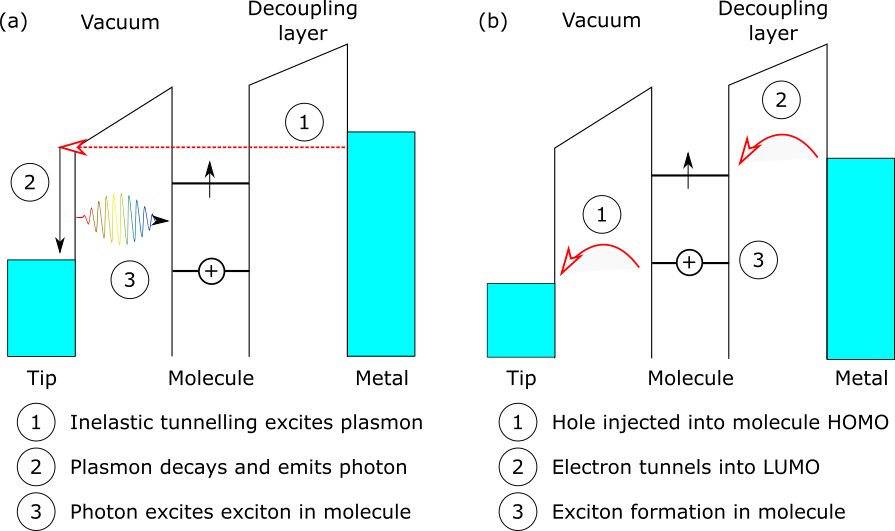
\includegraphics[width=0.9\textwidth]{pictures/exciton_mechanisms.png}
    \caption[Energy diagrams to describe two different emission mechanisms of an organic molecule. \textbf{(a)} Plasmon-mediated and \textbf{(b)} charge injection exciton formation.]{Energy diagrams to describe two different emission mechanisms of an organic molecule. \textbf{(a)} Plasmon-mediated and \textbf{(b)} charge injection exciton formation. Figure adapted from \citep{kuhnke2017atomic}. }
    \label{fig:exptech:2-mechanisms}
\end{figure}



\subsection{Experimental factors}

The success of an \ac{STML} experiment is dependent on many factors, such as the material of the tip and sample, the geometry of the tip, and the optical properties of the molecule.

For strong luminescence from tunnelling electrons, the tip and sample should be composed of materials with low dielectric loss in the wavelength region of interest. Organic semiconducting molecules typically have optical gaps of 1\SI{-3}{eV}, resulting in exciton emission in the visible/IR range. For \ac{STML} study of organic molecules should be performed with tip and sample composed of noble metals silver (Ag) \citep{yang2015optical} and gold (Au) \citep{olmon2012optical}. Low dielectric loss means that electric field can more easily penetrate the material, and the conduction electrons in the metal can move more freely within the bulk, allowing for stronger plasmonic response \citep{novotny2012principles}. Oxide layers or other contaminants can quench emissions from the tip-sample junction.

The tip geometry is crucial to maximizing signal-to-noise ratio in \ac{STML}. Luminescence signals can be enhanced by the plasmonic nano-cavity formed by the tip and the sample, an effect known as Purcell enhancement \citep{purcell1946spontaneous}. The coupling of the exciton and the plasmon can increase the strength of the organic molecule \ac{STML} signal by up to five orders of magnitude \citep{chen2015molecular}. Theoretical simulations have determined that stronger plasmonic response is seen in sharper tips due to the enhancement of electric fields at the tip apex by the lightning rod effect \citep{novotny2012principles, aizpurua2000role}. Experimentally, the exact tip geometry cannot be determined, however, small changes to the tip apex can change the energy and strength of the plasmon emission dramatically \citep{meguro2002origin}. For our experiment, the tip was pulsed and indented until the detected plasmon emission is strong and broad, extending into visible/IR spectral range. 

Additionally, the molecules should possess a high quantum photoluminescent efficiency, the ratio of photons emitted per charge carrier, and high stability on the surface, especially under the strong electromagnetic fields in the tip-sample junction. Regardless of prevalent mechanism for \ac{STML} on organic molecules, molecule-substrate interactions should be minimized to prevent quenching of luminescence due to additional energetic pathways for the excitation to relax \citep{kuhnke2017atomic, rossel2010fluorescence}. This is usually done by using a thin insulating layer between the molecule and substrate, such as metal-oxide or NaCl layers. 









\endinput








\subsection{garbage}
\begin{equation}
    I_t \propto e^{-2kz},
\end{equation}

where $k$ is 

Has proven to be powerful in understanding the topological and electronic features of surfaces near the atomic level. 

The works \citep{tersoff19931} of \textit{Young et al.}, with the creation of the topografiner, and \textit{Teague}, with the demonstration of vacuum tunnelling between gold electrodes, preceeded the invention of \ac{STM}. The topografiner used a piezoelectric driver to scan surfaces with a probe at small distances, advancing the technology required for the \ac{STM}. Teague's experiments revealed the possibility of vacuum tunnelling, at the voltages and gap widths used today in \ac{STM}. 

\ac{STM} is based on the quantum tunnelling of electrons through a potential barrier. In experiment, a tip is brought close to the sample of interest. A bias is applied to the system to allow for tunnelling, and the measured current gives information about the sample's \ac{LDOS}. The tip-sample distance is usually around 5 to 15 Angstroms, with the tunnelling current in the nano-ampere range. The voltage applied can range from 10mV to 10V in either directions.


Here, we notice that $P_t$ is the sinc function, which contributes to the integral mostly in the region of $[-2h/t, 2h/t]$. So as $t$ grows, the interval becomes smaller and smaller, until the tip energy $E_k$ can be approximated to be constantly distributed in the interval. The sum can then be approximated to be an integral, with $\rho_{tip}(\epsilon)$ being the number of tip states near the energy of the sample state $\epsilon$, 
\begin{align}
\sum_k P_t(E_k - \epsilon) \abs{\mathfrak{M}}^2 &\approx \abs{\mathfrak{M}}^2(\psi) \rho_{tip}(\epsilon) \int_{-2h/t}^{2h/t} P_t(E) dE \\
& \approx \abs{\mathfrak{M}}^2(\psi) \rho_{tip}(\epsilon) \int_{-\infty}^{\infty} P_t(E) dE = \abs{\mathfrak{M}}^2(\psi) \rho_{tip} \frac{\pi t}{2\hbar}.
\end{align}
Finally, the scattering rate (or the transition probability) is given by
\begin{equation}
\frac{d}{dt} \sum_k |a_k(t)|^2 \approx \frac{d}{dt}\left( \frac{2\pi t}{\hbar} \abs{\mathfrak{M}}^2(\psi) \rho_{tip}(\epsilon) \right) = \frac{2 \pi}{\hbar} \abs{\mathfrak{M}}^2(\psi) \rho_{tip}(\epsilon).
\end{equation}

can excite localised charge oscillations known as \acp{TIP} in metallic substrate. At the interface between the substrate and the vacuum, the \ac{TIP} mode can become electromagnetically coupled, creating \acp{SPP} which propagate parallel to the interface. Upon decay of the \ac{SPP}, photons are radiated. This process is dominant in 

Theoretical studies estimate the inelastic tunnelling accounts for about 1\% of the total current,  where elastic tunnelling dominates the signal. Of the \acp{TIP} generated by inelastic tunnelling, only about 10\% couple with the electromagnetic field, yielding photon counts of $\sim 10^{-4}$ per tunnelled carrier. To maximise this signal, there are two main experimental considerations: the shape of the tip, and the material of the tip and sample.
